\documentclass[aspectratio=169,12pt]{beamer}
\usepackage[utf8]{inputenc}
\usepackage{amsmath, amssymb}
\usepackage{booktabs}
\usepackage{colortbl}
\usepackage{hyperref}
\usepackage{makecell}
\usepackage{ragged2e}
\usepackage{bytefield}
\usepackage{tikz}
\usetikzlibrary{arrows.meta, positioning, shapes.geometric, calc, tikzmark, shapes.misc}
\usepackage{tcolorbox}
\usetheme{Madrid}
\title{Multithreading and Power}
\author{Computer Architecture 2340267}
\date{2025, Recitation \#12}

\begin{document}

\frame{\titlepage}

\begin{frame}{Outline}
\tableofcontents
\end{frame}

\section{Introduction to Execution Models}

\begin{frame}{Scalar Execution}
\begin{itemize}
    \item Sequential execution of instructions
    \item One instruction at a time
    \item Dependencies reduce throughput/utilization
\end{itemize}

\vspace{0.5cm}
\begin{center}
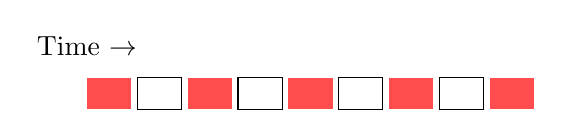
\begin{tikzpicture}[scale=0.8]
    \node at (0,0.5) {Time $\rightarrow$};
    \foreach \x in {0,0.8,1.6,2.4,3.2,4.0,4.8,5.6,6.4} {
        \pgfmathparse{int(mod(\x/0.8,2))}
        \ifnum\pgfmathresult=0
            \fill[red!70] (\x,0) rectangle (\x+0.7,-0.5);
        \else
            \draw (\x,0) rectangle (\x+0.7,-0.5);
        \fi
    }
\end{tikzpicture}
\end{center}

\begin{alertblock}{Key Issue}
Dependencies reduce throughput/utilization
\end{alertblock}
\end{frame}

\begin{frame}{Superscalar Execution}
\begin{itemize}
    \item Multiple instructions per cycle
    \item Out-of-order execution capabilities
    \item Still limited by:
    \begin{itemize}
        \item Dependencies
        \item Cache misses
        \item Branch mispredictions
    \end{itemize}
\end{itemize}

\begin{block}{Impact}
These factors reduce throughput/utilization even in superscalar processors
\end{block}
\end{frame}

\section{Multithreading Approaches}

\begin{frame}{Blocked Multithreading}
\framesubtitle{Switch on Event}

\begin{itemize}
    \item Switch threads when current thread encounters low utilization event
    \item Examples of switching events:
    \begin{itemize}
        \item L2 cache miss
        \item Long latency operations
    \end{itemize}
    \item May increase utilization and throughput
\end{itemize}

\begin{block}{Benefit}
Hides long latency events by switching to another thread
\end{block}
\end{frame}

\begin{frame}{Fine Grained Multithreading}
\begin{itemize}
    \item Switch threads frequently (e.g., every cycle)
    \item Reduces impact of dependencies
    \item Better latency hiding than blocked multithreading
\end{itemize}

\begin{block}{Key Advantage}
Increases utilization/throughput by reducing impact of dependencies
\end{block}
\end{frame}

\begin{frame}{Simultaneous Multithreading (SMT)}
\begin{columns}
\column{0.5\textwidth}
\begin{itemize}
    \item Multiple threads execute simultaneously
    \item Shares execution resources
    \item Best utilization of resources
\end{itemize}

\column{0.5\textwidth}
\begin{block}{Benefits}
\begin{itemize}
    \item Reduces impact of dependencies
    \item Hides cache misses
    \item Masks branch mispredictions
\end{itemize}
\end{block}
\end{columns}

\vspace{0.5cm}
\begin{center}
\textbf{Pipeline:} In-order fetch/decode/rename $\rightarrow$ Out-Of-Order Execution $\rightarrow$ In-order Retire
\end{center}
\end{frame}

\section{Performance Analysis}

\begin{frame}{Switch-on-Event Analysis}
\begin{columns}
\column{0.5\textwidth}
\textbf{Given Parameters:}
\begin{itemize}
    \item M instructions execute with cache access
    \item Cache miss takes Q cycles
    \item Thread switch on cache miss (event)
    \item $CPI_{ideal}$ when Thread 0 runs
    \item N threads available
\end{itemize}

\column{0.5\textwidth}
\textbf{Analysis:}
\begin{itemize}
    \item Each memory access: Q cycles
    \item Memory access every M instructions
    \item Context switch overhead considered
\end{itemize}
\end{columns}
\end{frame}

\begin{frame}{IPC Equation Development}
\textbf{Question:} Develop an equation for IPC as a function of running threads (N)

\begin{block}{CPI per Thread}
$$CPI_{Thread} = CPI_i + \frac{Q}{M}$$
\end{block}

Where:
\begin{itemize}
    \item $CPI_i$ = ideal CPI
    \item Q = memory access cycles
    \item M = instructions between memory accesses
\end{itemize}

\begin{alertblock}{IPC Formula}
$$IPC = \frac{N}{CPI_i + \frac{Q}{M}}$$
\end{alertblock}
\end{frame}

\begin{frame}{Performance Optimization}
\textbf{Best Achievable Performance:}
\begin{itemize}
    \item Maximum IPC when memory latencies are fully hidden
    \item Achieved when: No memory accesses OR all latencies masked by other threads
\end{itemize}

$$IPC_{max} = CPI_{ideal}^{-1}$$

\textbf{Minimum Threads for Maximum Performance:}
$$N_1 = 1 + \frac{Q}{M \cdot CPI_i}$$
\end{frame}

\begin{frame}{IPC vs Number of Threads}
\begin{center}
\begin{tikzpicture}[scale=0.8]
    \draw[->] (0,0) -- (8,0) node[right] {N = Threads};
    \draw[->] (0,0) -- (0,4.5) node[above] {IPC};
    
    % Draw roofline (not curve)
    \draw[thick, blue] (0,0) -- (3,3.5);
    \draw[thick, blue] (3,3.5) -- (7.5,3.5);
    
    % Mark key points
    \draw[dashed] (3,0) -- (3,3.5) node[pos=0, below] {$N_1$};
    \draw[dashed] (0,3.5) -- (3,3.5) node[pos=0, left] {$IPC_{Max}$};
    
    % Equation annotation
    \node at (5.5,2) {$IPC = \frac{N}{CPI_i + \frac{Q}{M}}$};
\end{tikzpicture}
\end{center}
\end{frame}

\section{Cache Impact}

\begin{frame}{L1 Cache Addition}
\textbf{Improvement Proposal:} Add L1 cache with 0 cycles access time

\begin{block}{Modified IPC with Cache}
$$IPC = \frac{N}{CPI_i + k \cdot \frac{Q}{M}} \quad \text{where } k = \text{miss rate (k = 1} \rightarrow \text{100\% miss rate)}$$
\end{block}

\textbf{Question:} What cache hit rate provides maximum performance with $N_1/2$ threads?
\begin{align*}
IPC_{Max} &= IPC_{ideal} & \Rightarrow N_1 = 1 + \frac{Q}{M \cdot CPI_i} \quad \Rightarrow \quad \frac{N_1}{2} = \frac{1 + \frac{Q}{M \cdot CPI_i}}{2}
\end{align*}

Solve: $IPC\Big|_{N=\frac{N_1}{2}} = \left(CPI_i + k \cdot \frac{Q}{M}\right)^{-1} \cdot \frac{1}{2} \cdot CPI_i^{-1} = CPI_i^{-1}$

\begin{tcolorbox}[colback=blue!5!white,colframe=blue!75!black]
$$CPI\left(\frac{N_1}{2}\right) = \left(CPI_i + Q \cdot \frac{k}{M}\right) \cdot \frac{2 \cdot M \cdot CPI_i}{M \cdot CPI_i + Q} = CPI_i$$
\end{tcolorbox}

\alert{Result: $k = 0.5$ (50\% miss rate) $\Rightarrow$ 50\% hit rate required}
\end{frame}

\begin{frame}{Cache Design Impact}
\textbf{How will cache addition affect the CPU?}

\begin{columns}
\column{0.30\textwidth}
\begin{block}{Area}
\textcolor{red}{Increase} \\
Cache requires silicon area
\end{block}

\column{0.30\textwidth}
\begin{block}{Power}
\textcolor{green}{Decrease} \\
(with sufficient hit rate)
\end{block}

\column{0.33\textwidth}
\begin{block}{Complexity}
\textcolor{red}{Increase} \\
Cache control logic needed
\end{block}
\end{columns}

\vspace{0.5cm}
\begin{itemize}
    \item Might allow CPU redesign with fewer threads if hit rate is high enough
\end{itemize}
\end{frame}


\section{Power/Performance Trade-offs}

\begin{frame}{Power/Performance Analysis}
\textbf{Two Processor Options:}

\begin{table}
\centering
\begin{tabular}{lcc}
\toprule
Parameter & Large Core & Small Core \\
\midrule
Area & 4 mm² & 2 mm² \\
Width & 4-wide & 2-wide \\
IPC & 2 & 1 \\
Leakage Power & ? & 0.5W \\
Dynamic Capacitance & 1500 pF & 500 pF \\
Threads & 1 & 1 \\
\bottomrule
\end{tabular}
\end{table}

\begin{block}{Key Assumption}
Leakage is approximately proportional to area
\end{block}

\textbf{Calculate large core leakage:}
$$\text{Leakage}_{\text{big core}} = \frac{\text{area}_{\text{big core}}}{\text{area}_{\text{small core}}} \times \text{Leakage}_{\text{small core}} = \frac{4}{2} \times 0.5\text{W} = 1\text{W}$$
\end{frame}

\begin{frame}{Voltage-Frequency Operating Points}
\begin{table}
\centering
\small
\begin{tabular}{ccc}
\toprule
Voltage (V) & Large Core Freq (GHz) & Small Core Freq (GHz) \\
\midrule
0.6 & 0.7 & 1.0 \\
0.65 & 1.0 & 1.25 \\
0.7 & 1.35 & 1.5 \\
0.75 & 1.75 & 1.75 \\
0.8 & 2.25 & 2.0 \\
0.85 & 2.5 & 2.25 \\
0.9 & 3.0 & 2.5 \\
0.95 & 3.5 & 2.75 \\
1.0 & 4.0 & 3.0 \\
\bottomrule
\end{tabular}
\end{table}
\end{frame}

\subsection{Single Thread Performance}

\begin{frame}{Single Thread Performance (4W Budget)}
\textbf{Question:} Which processor for best single-thread performance at 4W?

\begin{block}{Power Equation}
$$Power = Leakage + CV^2f$$
\end{block}

\textbf{Analysis:}
\begin{itemize}
    \item Small core: Can run at 3 GHz within 4W
    \item Large core: Can run at 2.5 GHz within 4W
\end{itemize}

\textbf{Performance (approx. $\propto$ F × IPC):}
\begin{itemize}
    \item Small: $1 \times 3 = 3$ G inst/sec
    \item Large: $2 \times 2.5 = 5$ G inst/sec
\end{itemize}

\alert{Result: Large core provides better performance}
\end{frame}

\subsection{Multi-Thread Performance}

\begin{frame}{Multi-Thread Performance (2W per Core)}
\textbf{Question:} Two large cores or two small cores for best 2-way MT performance?

\textbf{Power constraint:} 2W per core

\textbf{Operating Points:}
\begin{itemize}
    \item Small cores: 3 GHz each
    \item Large cores: 1.35 GHz each
\end{itemize}

\textbf{Performance (approx. $\propto$ N × F × IPC):}
\begin{itemize}
    \item 2 Small: $2 \times 3 \times 1 = 6$ G inst/sec
    \item 2 Large: $2 \times 1.35 \times 2 = 5.4$ G inst/sec
\end{itemize}

\alert{Result: Two small cores provide better performance}
\end{frame}

\begin{frame}{Power Table Analysis (2W per Core)}
\textbf{Question:} Given a 2W power budget per core, which configuration provides best 2-way Multi-Thread performance: two large cores or two small cores?
\vspace{3mm}
\begin{columns}[t]
\column{0.6\textwidth}
\scriptsize
\begin{tabular}{|c|c|c|c|c|c|c|}
\hline
\makecell{Voltage \\ (V)} &
\makecell{Freq \\ Large \\ Core \\ (GHz)} &
\makecell{Freq \\ Small \\ Core \\ (GHz)} &
\makecell{$P_{act}$ \\ Large \\ Core \\ (W)} &
\makecell{$P_{act}$ \\ Small \\ Core \\ (W)} &
\makecell{$P_{tot}$ \\ Large \\ Core \\ (W)} &
\makecell{$P_{tot}$ \\ Small \\ Core \\ (W)} \\
\hline
0.6 & 0.7 & 1 & 0.38 & 0.18 & 1.38 & 0.68 \\
0.65 & 1 & 1.25 & 0.63 & 0.26 & 1.63 & 0.76 \\
0.7 & \tikzmark{lgf1}1.35\tikzmark{lgf2} & 1.5 & 0.99 & 0.37 & \tikzmark{lg1}1.99\tikzmark{lg2} & 0.87 \\
0.75 & 1.75 & 1.75 & 1.48 & 0.49 & 2.48 & 0.99 \\
0.8 & 2.25 & 2 & 2.16 & 0.64 & 3.16 & 1.14 \\
0.85 & 2.5 & 2.25 & 2.71 & 0.81 & 3.71 & 1.31 \\
0.9 & 3 & 2.5 & 3.65 & 1.01 & 4.65 & 1.51 \\
0.95 & 3.5 & 2.75 & 4.74 & 1.24 & 5.74 & 1.74 \\
1 & 4 & \tikzmark{smf1}3\tikzmark{smf2} & 6.00 & 1.50 & 7.00 & \tikzmark{sm1}2.00\tikzmark{sm2} \\
\hline
\end{tabular}

\pause


\begin{tikzpicture}[remember picture, overlay]
% Oval for large core frequency (wider)
\draw[red, thick] ([xshift=2mm, yshift=1mm]pic cs:lgf1) ellipse (4mm and 2mm);
% Oval for large core power (wider)
\draw[red, thick] ([xshift=2mm, yshift=1mm]pic cs:lg1) ellipse (4mm and 2mm);
% Arrow connecting them - from east of frequency to west of power
\draw[red, thick, ->] ([xshift=6mm, yshift=1mm]pic cs:lgf1) -- ([xshift=-4mm,yshift=1mm]pic cs:lg1);

% Oval for small core frequency (wider)
\draw[red, thick] ([xshift=2mm,yshift=1mm]pic cs:smf1) ellipse (4mm and 2mm);
% Oval for small core power (wider)
\draw[red, thick] ([xshift=2mm,yshift=1mm]pic cs:sm1) ellipse (4mm and 2mm);
% Arrow connecting them - from east of frequency to west of power
\draw[red, thick, ->] ([xshift=6mm, yshift=1mm]pic cs:smf1) -- ([xshift=-4mm, yshift=1mm]pic cs:sm1);
\end{tikzpicture}

\column{0.4\textwidth}
\pause

\vspace{-2.3cm}
\textbf{Answer:}

\textbf{Small cores:}
\begin{itemize}
    \item Run at 3 GHz
    \item Perf: $2 \times 3 \times 1 = 6$ G inst/sec
\end{itemize}

\textbf{Large cores:}
\begin{itemize}
    \item Run at 1.35 GHz
    \item Perf: $2 \times 1.35 \times 2 = 5.4$ G inst/sec
\end{itemize}

\alert{Two small cores are better}
\end{columns}
\end{frame}

\begin{frame}{Power Curve Characteristics}
\begin{columns}
\column{0.45\textwidth}
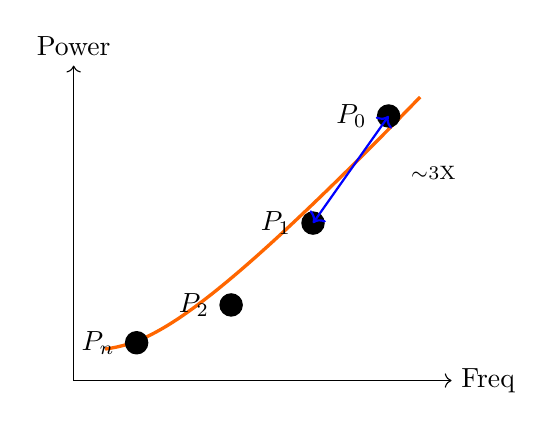
\begin{tikzpicture}[scale=0.8]
    \draw[->] (0,0) -- (6,0) node[right] {Freq};
    \draw[->] (0,0) -- (0,5) node[above] {Power};

    % Draw power curve - orange, steeper cubic relationship
    \draw[thick, orange!80!red, line width=1.2pt] (0.5,0.5) .. controls (1.2,0.6) and (2,0.9) .. (5.5,4.5);

    % Mark points from bottom to top
    \node[circle,fill=black,inner sep=3pt,label=left:$P_n$] at (1,0.6) {};
    \node[circle,fill=black,inner sep=3pt,label=left:$P_2$] at (2.5,1.2) {};
    \node[circle,fill=black,inner sep=3pt,label=left:$P_1$] at (3.8,2.5) {};
    \node[circle,fill=black,inner sep=3pt,label=left:$P_0$] at (5,4.2) {};

    % Arrow and annotation for P1 to P0
    \draw[<->,blue,thick] (3.8,2.5) -- (5,4.2);
    \node[right,align=left,font=\scriptsize] at (5.2,3.3) {$\sim$3X};
\end{tikzpicture}

\column{0.55\textwidth}
\textbf{At $P_n$ ($V_{min}$ = Energy efficient point):}
\begin{itemize}\small
    \item Freq decrease doesn't decrease V: $P \propto K \cdot F$
    \item Freq decrease by 1\% decreases power by 1\%
    \item Perf. features better than 1:1
\end{itemize}

\vspace{0.3cm}
\textbf{At $P_2$ (mid-range):}
\begin{itemize}\small
    \item Perf. features better than 1:3
    \item (1\% perf / less than 3\% power)
\end{itemize}

\vspace{0.3cm}
\textbf{Key relationships:}
\begin{itemize}\small
    \item $P = CV^2f$; $f = KV \Rightarrow P \propto f^3$
    \item $E = P \times t \Rightarrow E \propto f^2$
\end{itemize}
\end{columns}
\end{frame}

\begin{frame}{Summary}
\begin{itemize}
    \item \textbf{Multithreading} improves processor utilization
    \item \textbf{SMT} provides best resource utilization
    \item \textbf{IPC} increases with thread count up to saturation
    \item \textbf{Cache} can reduce required thread count
    \item \textbf{Power/Performance} trade-offs depend on workload:
    \begin{itemize}
        \item Single-thread: Large cores often better
        \item Multi-thread: Small cores can be more efficient
    \end{itemize}
    \item \textbf{Energy efficiency} achieved at moderate frequencies
\end{itemize}
\end{frame}

\end{document}